%=========================================================================
%  CHE F313 - Separation Processes II
%  PROBLEMS AND SOLUTIONS
%
%  Every numerical question in the uploaded material:
%    Part A  the eight lecture decks            (Slides/)
%    Part B  Tutorial 3 and Tutorial 4          (Tutorials/)
%    Part C  Quiz-1 and Tutorial Test 1         (Tests/)
%
%  Questions are quoted from those files; the solution method for each one
%  is the method taught in the lecture that set it.
%
%  Compile:  latexmk -xelatex SP2-Problems-and-Solutions.tex
%=========================================================================
\documentclass[10pt,a4paper]{article}

\usepackage[a4paper,left=18mm,right=18mm,top=15mm,bottom=17mm]{geometry}
\usepackage[T1]{fontenc}
\usepackage{amsmath,amssymb,mathtools}
\usepackage{xcolor}
\usepackage{booktabs,tabularx,array,multirow}
\usepackage{enumitem}
\usepackage{fancyhdr}
\usepackage{tcolorbox}
\tcbuselibrary{breakable,skins}
\usepackage{graphicx}
\usepackage{siunitx}
\usepackage[colorlinks=true,linkcolor=accent,urlcolor=accent2]{hyperref}

\definecolor{accent}{HTML}{0B3C5D}
\definecolor{accent2}{HTML}{1D6FA5}
\definecolor{qframe}{HTML}{1B5E20}
\definecolor{qbg}{HTML}{EAF5EC}
\definecolor{mframe}{HTML}{1D6FA5}
\definecolor{mbg}{HTML}{EAF1F8}
\definecolor{boxbg}{HTML}{F1F4F7}
\definecolor{rule}{HTML}{9FB3C2}
\definecolor{inbox}{HTML}{0E2430}
\definecolor{notecol}{HTML}{46535C}
\definecolor{warncol}{HTML}{8E2B0F}
\definecolor{warnbg}{HTML}{FDF2EC}

\sisetup{detect-all,per-mode=symbol}
\newcommand{\microm}{\ensuremath{\,\mu\mathrm{m}}}

\newtcolorbox{qbox}{breakable,enhanced,colback=qbg,colframe=qframe!65,
  boxrule=0.6pt,arc=1.5pt,left=6pt,right=6pt,top=4pt,bottom=4pt,
  before skip=5pt,after skip=4pt,fontupper=\small}
\newtcolorbox{mthbox}{breakable,enhanced,colback=mbg,colframe=mframe!65,
  boxrule=0.6pt,arc=1.5pt,left=6pt,right=6pt,top=4pt,bottom=4pt,
  before skip=5pt,after skip=4pt,fontupper=\small}
\newtcolorbox{ansbox}{enhanced,colback=boxbg,colframe=accent,boxrule=0.9pt,
  arc=1.5pt,left=6pt,right=6pt,top=5pt,bottom=5pt,before skip=5pt,after skip=6pt,
  fontupper=\small\color{inbox}}
\newtcolorbox{warnbox}{breakable,enhanced,colback=warnbg,colframe=warncol!60,
  boxrule=0.6pt,arc=1.5pt,left=6pt,right=6pt,top=4pt,bottom=4pt,
  before skip=5pt,after skip=4pt,fontupper=\small}

\newcommand{\spsection}[1]{%
  \par\addvspace{10pt}%
  \noindent\begin{tcolorbox}[colback=accent,colframe=accent,boxrule=0pt,arc=1.2pt,
      left=7pt,right=7pt,top=5pt,bottom=5pt,width=\linewidth,before skip=0pt,after skip=7pt]
    \color{white}\bfseries\large #1
  \end{tcolorbox}\par\vspace{-2pt}\nopagebreak}
\newcommand{\spsub}[1]{\par\addvspace{7pt}\noindent{\color{accent}\bfseries #1}\par\addvspace{3pt}\nopagebreak}
\newcommand{\qtitle}[2]{%
  \par\addvspace{9pt}\noindent
  \begin{tcolorbox}[colback=accent2!12,colframe=accent2,boxrule=0.8pt,arc=1.5pt,
      left=7pt,right=7pt,top=4pt,bottom=4pt,before skip=0pt,after skip=4pt,width=\linewidth]
    {\large\bfseries\color{accent}#1}\hfill{\small\color{accent2}#2}
  \end{tcolorbox}\par\vspace{1pt}}
\newcommand{\src}[1]{\par\vspace{1pt}\noindent{\small\color{notecol}\textbf{Source:} #1}\par\vspace{3pt}}
\newcommand{\note}[1]{\par\vspace{1pt}\noindent{\small\color{notecol}#1}\par\vspace{2pt}}

\setlist[itemize]{leftmargin=1.2em,topsep=2pt,itemsep=1.5pt,parsep=0pt}
\setlist[enumerate]{leftmargin=1.6em,topsep=2pt,itemsep=1.5pt}
\setlength{\parindent}{0pt}
\setlength{\parskip}{2.5pt}
\emergencystretch=2em

\pagestyle{fancy}
\fancyhf{}
\renewcommand{\headrulewidth}{0pt}
\renewcommand{\footrulewidth}{0.4pt}
\fancyfoot[L]{\footnotesize\color{notecol}CHE F313 \textperiodcentered{} Problems \& Solutions}
\fancyfoot[R]{\footnotesize\color{notecol}Page \thepage}

\begin{document}

\begin{center}
{\LARGE\bfseries\color{accent} SEPARATION PROCESSES II}\\[2pt]
{\color{accent2} CHE F313 \textperiodcentered{} Problems and Solutions \textperiodcentered{} I-Semester 2026-27}\\[4pt]
{\color{rule}\rule{0.6\linewidth}{0.8pt}}\\[6pt]
{\large\bfseries\color{accent} Every numerical question in the uploaded material, with its solution}\\[3pt]
{\color{accent2} Part A: lecture decks \textperiodcentered{} Part B: tutorials \textperiodcentered{} Part C: quiz and tutorial test}
\end{center}

\vspace{1mm}
Every question below is quoted from one of the uploaded files, and every solution uses the
method taught in the lecture that set it. The questions are grouped by source:

\begin{itemize}
  \item \textbf{Part A --- lecture decks} (\texttt{Slides/}): Mod 1 Lec 2, Mod 1 Lec 3, Mod 1 Lec 4, Mod 1 Lec 5, Mod 2 Lec 1.
  \item \textbf{Part B --- tutorials} (\texttt{Tutorials/}): Tutorial 3 (01-09-2026), Tutorial 4 (07-09-2026).
  \item \textbf{Part C --- tests} (\texttt{Tests/}): Quiz-1 (03-09-2026), Tutorial Test 1 (07-09-2026).
\end{itemize}

\spsub{Question inventory}
{\small
\begin{tabularx}{\linewidth}{@{}l l X l@{}}
\toprule
\textbf{ID} & \textbf{Source} & \textbf{Topic} & \textbf{Solved at}\\
\midrule
Q1 & Mod 1 Lec 3, slide 10 & Clay catalyst: differential \& cumulative analysis, $A_w$, $\overline{D}_s$, particle count & p.\,\pageref{q:1}\\
Q2 & Mod 1 Lec 3, slides 11--12 (table on 12) & Crushed quartz: $A_w$, $N_w$, $\overline{D}_v$, $\overline{D}_s$, $\overline{D}_w$, $N_i$, number fraction & p.\,\pageref{q:2}\\
Q3 & Mod 1 Lec 4, slide 19 & Muller mixer: mixing index $I_p$ and standard deviation & p.\,\pageref{q:3}\\
Q4 & Mod 1 Lec 5, slide 20 & Crusher power by Rittinger's law & p.\,\pageref{q:4}\\
Q5 & Mod 2 Lec 1, slide 16 & Quartz screened at 10 mesh: $D/F$, $B/F$, overall effectiveness $E$ & p.\,\pageref{q:5}\\
Q6 & Tutorial 3, Problem 1 & Sieve analysis: differential \& cumulative curves, $D_{50}$, particle counts, $A_w$ & p.\,\pageref{q:6}\\
Q7 & Tutorial 3, Problem 2 & Shape factor and sphericity of an irregular particle & p.\,\pageref{q:7}\\
Q8 & Tutorial 4, Problem 1 & Crusher power when capacity and product size change & p.\,\pageref{q:8}\\
Q9 & Tutorial 4, Problem 2 & Energy per kg of material (Kick's law) & p.\,\pageref{q:9}\\
Q10 & Quiz-1, 03-09-2026 & Mixing index of a binary solid mixture from ten samples & p.\,\pageref{q:10}\\
Q11 & Tutorial Test 1, 07-09-2026 & Bond work index and the power for a finer product & p.\,\pageref{q:11}\\
\bottomrule
\end{tabularx}}

\note{Parts of Q2, Q6, Q7, Q8, Q9 and Q11 sit inside pictures on the source slides rather than in
their text; those parts were read from the pictures and are quoted as printed. Where a source leaves
something undefined, the note at the end of that solution says so instead of filling it in.}

\newpage
\spsection{PART A --- PROBLEMS IN THE LECTURE DECKS}

\qtitle{Q1 --- Screen analysis of a clay catalyst}{Module 1 \textperiodcentered{}\label{q:1} Lecture 3 \textperiodcentered{} slide 10}
\src{\texttt{Slides/Mod1-Lecture 3.pptx}, slide 10 (``Problem 1: Screen Analysis'')}

\begin{qbox}
``Finely divided clay is used as a catalyst in the petroleum industry. It has density of 1.2\,g/cc and
a sphericity of 0.5. The size analysis is as follows:''
\begin{center}\small
\begin{tabular}{@{}l S[table-format=1.4] S[table-format=1.4] S[table-format=1.4] S[table-format=1.4] S[table-format=1.4]@{}}
\toprule
$D_{pi}$ / \si{\milli\meter} & 0.0252 & 0.0178 & 0.0126 & 0.0089 & 0.0038\\
$x_i$ (g/g) & 0.088 & 0.178 & 0.293 & 0.194 & 0.247\\
\bottomrule
\end{tabular}
\end{center}
``Show the differential \& cumulative screen analysis of the mixture. Find the specific surface area
and the Sauter mean diameter of the clay material. Find the number of particles in 1\,g sample.''
\end{qbox}

\begin{mthbox}
\textbf{Method from the slides.} Specific surface area and mean diameters (Mod 1 Lec 3):
\[
A_w=\frac{6}{\rho_p\Phi_s}\sum_{i=1}^{n}\frac{x_i}{D_{pi}},\qquad
\overline{D}_s=\frac{1}{\sum_i x_i/D_{pi}}=\frac{6}{\Phi_s\rho_p A_w},\qquad
N_w=\frac{1}{a\rho_p}\sum_{i=1}^{n}\frac{x_i}{D_{pi}^3}
\]
Cumulative analysis is built by adding the increments consecutively, starting from the smallest
particles (Mod 1 Lec 2, slide 16).
\end{mthbox}

\spsub{Solution}
\textbf{1. Differential and cumulative analysis.} The differential analysis is the tabulated $x_i$
against $D_{pi}$. The cumulative ``fraction smaller than $D_{pi}$'' is the running sum from the
smallest size; ``fraction larger'' is its complement. Check: $\sum x_i=1.000$.
\begin{center}\small
\begin{tabular}{@{}S[table-format=1.4] S[table-format=1.3] S[table-format=1.4] S[table-format=1.4]@{}}
\toprule
{$D_{pi}$ / \si{\milli\meter}} & {$x_i$} & {cumulative smaller} & {cumulative larger}\\
\midrule
0.0038 & 0.247 & 0.2470 & 0.7530\\
0.0089 & 0.194 & 0.4410 & 0.5590\\
0.0126 & 0.293 & 0.7340 & 0.2660\\
0.0178 & 0.178 & 0.9120 & 0.0880\\
0.0252 & 0.088 & 1.0000 & 0.0000\\
\bottomrule
\end{tabular}
\end{center}

\textbf{2. Specific surface area and Sauter mean diameter.} With
$\rho_p=\SI{1.2}{\gram\per\cubic\centi\meter}=\SI{1.2e-3}{\gram\per\cubic\milli\meter}$ and
$\Phi_s=0.5$:
\[
\sum_i\frac{x_i}{D_{pi}}=123.544\ \text{mm}^{-1},\qquad
A_w=\frac{6}{(\num{1.2e-3})(0.5)}(123.544)=\SI{1.2354e6}{\square\milli\meter\per\gram}
=\SI{1.24}{\square\meter\per\gram}
\]
\[
\overline{D}_s=\frac{1}{123.544}=\SI{0.008094}{\milli\meter}=\SI{8.09}{\micro\meter}
\]

\textbf{3. Number of particles in a \SI{1}{\gram} sample.} With $\sum x_i/D_{pi}^3=4.9601\times10^{6}\ \text{mm}^{-3}$,
\[
N_w=\frac{1}{a\rho_p}\sum_i\frac{x_i}{D_{pi}^3}=\frac{4.9601\times10^{6}}{a(\num{1.2e-3})}
=\frac{4.133\times10^{9}}{a}\ \text{particles per gram}
\]
For spheres, $a=\pi/6=0.5236$, giving $N_w=\SI{7.89e9}{particles\per\gram}$.

\begin{ansbox}
\textbf{(a)} $\sum x_i=1.000$; differential and cumulative tables as above.\\
\textbf{(b)} $A_w=\SI{1.2354e6}{\square\milli\meter\per\gram}=\SI{1.24}{\square\meter\per\gram}$;\quad
$\overline{D}_s=\SI{8.09}{\micro\meter}$.\\
\textbf{(c)} $N_w=(4.133\times10^{9})/a$ particles per gram; with $a=\pi/6$,
$N_w\approx\SI{7.9e9}{particles\per\gram}$.
\end{ansbox}

\begin{warnbox}
\textbf{Note.} The slide does not give the volume shape factor $a$ (unlike Q2, where $a=0.8$ is
stated). The value above assumes the sphere value $a=\pi/6$. Since $N_w\propto 1/a$, quoting $a$
from the question paper changes the answer: $a=0.5\to\SI{8.3e9}{\per\gram}$,
$a=0.8\to\SI{5.2e9}{\per\gram}$. Confirm the intended $a$ before submitting.
\end{warnbox}

\newpage
\qtitle{Q2 --- Screen analysis of crushed quartz}{Module 1 \textperiodcentered{}\label{q:2} Lecture 3 \textperiodcentered{} slides 11--12}
\src{\texttt{Slides/Mod1-Lecture 3.pptx}, slides 11--12 (``Problem 2: Screen Analysis''; the table sits on slide 12, headed \texttt{Numerical Problem}, and the same table appears on Lecture 2 slide 17)}

\begin{qbox}
``The screen analysis shown in Table applies to a sample of crushed quartz. The density of the
particles is 2650\,kg/m3 (0.00265\,g/mm3), and the shape factors are a = 0.8 and $\Phi_s = 0.571$.
For the material between 4-mesh and 200-mesh in particle size, calculate (a) Aw in square millimeters
per gram and Nw in particles per gram, (b) Dv (c) Ds (d) Dw and (e) Ni for the 150/200-mesh
increment. (f) What fraction of the total number of particles is in the 150/200-mesh increment?''
\end{qbox}

\begin{qbox}
\textbf{Table as printed on slide 12.} Columns: mesh, screen opening, mass fraction retained $x_i$,
average particle diameter in increment, cumulative fraction smaller than $D_{pi}$.
\begin{center}\footnotesize
\begin{tabular}{@{}l S[table-format=1.3] S[table-format=1.4] S[table-format=1.3] S[table-format=1.4]@{}}
\toprule
{Mesh} & {opening / \si{\milli\meter}} & {retained $x_i$} & {$D_{pi}$ in increment / \si{\milli\meter}} & {cumulative smaller}\\
\midrule
4 & 4.699 & 0.0000 & {---} & 1.0000\\
6 & 3.327 & 0.0251 & 4.013 & 0.9749\\
8 & 2.362 & 0.1250 & 2.845 & 0.8499\\
10 & 1.651 & 0.3207 & 2.007 & 0.5292\\
14 & 1.168 & 0.2570 & 1.409 & 0.2722\\
20 & 0.833 & 0.1590 & 1.001 & 0.1132\\
28 & 0.589 & 0.0538 & 0.711 & 0.0594\\
35 & 0.417 & 0.0210 & 0.503 & 0.0384\\
48 & 0.295 & 0.0102 & 0.356 & 0.0282\\
65 & 0.208 & 0.0077 & 0.252 & 0.0205\\
100 & 0.147 & 0.0058 & 0.178 & 0.0147\\
150 & 0.104 & 0.0041 & 0.126 & 0.0106\\
200 & 0.074 & 0.0031 & 0.089 & 0.0075\\
Pan & {---} & 0.0075 & 0.037 & 0.0000\\
\bottomrule
\end{tabular}
\end{center}
\end{qbox}

\begin{mthbox}
\textbf{Method from the slides.}
\[
A_w=\frac{6}{\rho_p\Phi_s}\sum\frac{x_i}{D_{pi}},\quad
N_w=\frac{1}{a\rho_p}\sum\frac{x_i}{D_{pi}^3},\quad
\overline{D}_v=\Big[\frac{1}{\sum x_i/D_{pi}^3}\Big]^{1/3},\quad
\overline{D}_s=\frac{1}{\sum x_i/D_{pi}},\quad
\overline{D}_w=\sum x_iD_{pi}
\]
and, for one increment, $N_i=\dfrac{x_i}{a\rho_p\overline{D}_{pi}^{3}}$ per unit mass of the whole sample.
\end{mthbox}

\spsub{Solution}
\textbf{Check of the table.} Each increment diameter is the mean of its two defining screen openings,
rounded to the three decimals printed: $(4.699+3.327)/2=4.013$, $(3.327+2.362)/2=2.845$, \dots,
$(0.074+0)/2=0.037$ for the pan. All 13 values agree to within \SI{0.0005}{\milli\meter}.

\textbf{The two sums (12 increments, 4-mesh to 200-mesh; pan excluded, since the question says
``between 4-mesh and 200-mesh''):}
\[
\sum_{i=1}^{12}\frac{x_i}{D_{pi}}=0.82780\ \text{mm}^{-1},\qquad
\sum_{i=1}^{12}\frac{x_i}{D_{pi}^3}=8.7932\ \text{mm}^{-3}
\]
(work for the first increment, $D_{pi}=4.013$, $x_i=0.0251$: $0.0251/4.013=0.00626$ and
$0.0251/4.013^3=0.000389$.)

\textbf{(a)}
\[
A_w=\dfrac{6}{(\num{2.65e-3})(0.571)}(0.82780)=\SI{3282}{\square\milli\meter\per\gram}
=\SI{32.8}{\square\centi\meter\per\gram},
\]
\[
N_w=\dfrac{8.7932}{(0.8)(\num{2.65e-3})}=\SI{4148}{particles\per\gram}.
\]

\textbf{(b)--(d)} $\overline{D}_v=[1/8.7932]^{1/3}=\SI{0.4845}{\milli\meter}$;\quad
$\overline{D}_s=1/0.82780=\SI{1.2080}{\milli\meter}$;\quad
$\overline{D}_w=\sum x_iD_{pi}=\SI{1.6775}{\milli\meter}$.

\textbf{(e)} For the 150/200-mesh increment $x_i=0.0031$ and $D_{pi}=\SI{0.089}{\milli\meter}$:
\[
N_i=\frac{0.0031}{(0.8)(\num{2.65e-3})(0.089)^3}=\SI{2074}{particles\per\gram}
\]

\textbf{(f)} The share of all particles in that increment is its share of $\sum x_i/D_{pi}^3$:
\[
\frac{N_i}{N_T}=\frac{0.0031/0.089^3}{8.7932}=0.5001\ \approx\ 50\%
\]
Compare its \emph{mass} fraction, $x_i=0.31\%$: half of all the particles sit in this one fine
increment although it is a negligible part of the mass.

\begin{ansbox}
\textbf{(a)} $A_w=\SI{3282}{\square\milli\meter\per\gram}$, \quad $N_w=\SI{4148}{particles\per\gram}$.\\
\textbf{(b)} $\overline{D}_v=\SI{0.484}{\milli\meter}$.\quad
\textbf{(c)} $\overline{D}_s=\SI{1.208}{\milli\meter}$.\quad
\textbf{(d)} $\overline{D}_w=\SI{1.677}{\milli\meter}$.\\
\textbf{(e)} $N_i=\SI{2074}{particles\per\gram}$.\quad
\textbf{(f)} $N_i/N_T=0.500$ --- about \textbf{50\%} of all particles, against 0.31\% of the mass.
\end{ansbox}

\begin{warnbox}
\textbf{Notes.}
\begin{itemize}
  \item \textbf{Scope.} Excluding the pan gives $\sum x_i=0.9925$, so the sums are not normalised to
        one. Including the pan instead gives $A_w=\SI{4086}{\square\milli\meter\per\gram}$,
        $N_w=\SI{73990}{particles\per\gram}$, $\overline{D}_v=\SI{0.185}{\milli\meter}$,
        $\overline{D}_s=\SI{0.970}{\milli\meter}$, $\overline{D}_w=\SI{1.678}{\milli\meter}$ and
        $N_i/N_T=2.8\%$. The exclusion follows the wording of the question.
  \item \textbf{Which diameter.} The increment means $D_{pi}$ from the table are used throughout; for
        the 150/200 increment that is $0.089$\,mm, not the screen openings $0.104$ or $0.074$\,mm.
\end{itemize}
\end{warnbox}

\newpage
\qtitle{Q3 --- Mixing index in a muller mixer}{Module 1 \textperiodcentered{}\label{q:3} Lecture 4 \textperiodcentered{} slide 19}
\src{\texttt{Slides/Mod1-Lecture 4.pptx}, slide 19 (``Problem 1'')}

\begin{qbox}
``A silty soil containing 14 percent moisture was mixed in a large muller mixer with 10\,wt\% of a
tracer consisting of dextrose and picric acid. After 3\,min of mixing, 12 random samples were taken
from the mix and analyzed calorimetrically for tracer material. The measured concentrations in the
sample were in weight percent tracer, 10.24, 9.30, 7.94, 10.24, 11.08, 10.03, 11.91, 9.72, 9.20,
10.76, 10.97, 10.55. Calculate the mixing index IP and the standard deviation.''
\end{qbox}

\begin{mthbox}
\textbf{Method from the slides} (cohesive solids / pastes, Mod 1 Lec 4 slides 16 and 18):
\[
s=\sqrt{\frac{\sum_{i=1}^{N}(x_i-\bar{x})^2}{N-1}}
=\sqrt{\frac{\sum_{i=1}^{N}x_i^2-\bar{x}\sum_{i=1}^{N}x_i}{N-1}},
\qquad
\sigma_0=\sqrt{\mu(1-\mu)},
\qquad
I_s=\frac{\sigma_0}{s}
\]
with $x_i$ the mass fraction of A in each sample, $\bar x$ their average, $N$ the number of spot
samples, and $\sigma_0$ the standard deviation at zero mixing.
\end{mthbox}

\spsub{Solution}
\[
\bar{x}=\frac{121.94}{12}=10.1617\ \text{wt\%},\qquad
\sum_{i=1}^{12}(x_i-\bar x)^2=11.890\ (\text{wt\%})^2
\]
\[
s=\sqrt{\frac{11.890}{12-1}}=\SI{1.0397}{wt\%}=0.010397\ \text{(mass fraction)}
\]
With the \SI{10}{wt\%} of tracer charged, $\mu=0.10$ and
\[
\sigma_0=\sqrt{0.10\times0.90}=0.30,
\qquad
I_p=\frac{0.30}{0.010397}=28.9
\]
A value of $I_p$ far above 1 shows a mixture much more uniform than a segregated charge, which is
the expected direction as mixing proceeds.

\begin{ansbox}
$\bar x=10.16$\,wt\%,\quad $s=\SI{1.04}{wt\%}$ ($0.0104$ as a mass fraction),\quad
$\sigma_0=0.30$,\quad $I_p=0.30/0.0104=28.9\approx 29$.
\end{ansbox}

\begin{warnbox}
\textbf{Notes.}
\begin{itemize}
  \item Using the measured mean instead of the charged composition, $\mu=\bar x=0.1016$, gives
        $\sigma_0=0.3022$ and $I_p=29.1$; using the $N$ denominator gives $s=\SI{0.995}{\percent}$ and
        $I_p=30.1$.
  \item The granular-solid form $\sigma_e=\sqrt{\mu_p(1-\mu_p)/n}$ cannot be used here: it needs $n$,
        the number of particles per sample, which the slide does not give.
  \item The slide writes the paste mixing index as $I_s$; the question calls it $I_p$. They are the
        same quantity.
\end{itemize}
\end{warnbox}

\newpage
\qtitle{Q4 --- Crusher power by Rittinger's law}{Module 1 \textperiodcentered{}\label{q:4} Lecture 5 \textperiodcentered{} slide 20}
\src{\texttt{Slides/Mod1-Lecture 5.pptx}, slide 20 (``Problem 1: Size reduction'')}

\begin{qbox}
``Particles of the average feed size of $50\times10^{-4}$\,m are crushed to an average product size
of $10\times10^{-4}$\,m at the rate of 20 tonnes per hour. At this rate, the crusher consumes
40\,kW of power which 5\,kW are required for running the mill empty. Calculate the power consumption
if 12 tonnes/h of this product is crushed to $5\times10^{-4}$\,m size in the same mill? Assume
Rittinger's Law is applicable.''
\end{qbox}

\begin{mthbox}
\textbf{Method fixed by the slide} (Mod 1 Lec 5, Rittinger's law):
\[
\frac{P}{\dot m}=K_R\Big[\frac{1}{\overline{D}_{Sb}}-\frac{1}{\overline{D}_{Sa}}\Big]
\]
with $\overline{D}_{Sa}$ the feed size and $\overline{D}_{Sb}$ the product size. The question directs
Rittinger's law, so Kick's and Bond's laws are not used.
\end{mthbox}

\spsub{Solution}
\textbf{1. Useful power of the first duty.} Of the \SI{40}{\kilo\watt} drawn, \SI{5}{\kilo\watt} runs
the mill empty:
\[
P_{\text{net},1}=40-5=\SI{35}{\kilo\watt}\ \text{at}\ \SI{20}{\tonne\per\hour},
\qquad
\frac{P_{\text{net},1}}{\dot m_1}=\SI{1.75}{\kilo\watt\hour\per\tonne}
\]

\textbf{2. Rittinger constant of this mill and material.}
\[
\frac{1}{D_{Sb}}-\frac{1}{D_{Sa}}=\frac{1}{10\times10^{-4}}-\frac{1}{50\times10^{-4}}
=1000-200=\SI{800}{\per\meter},
\qquad
K_R=\frac{1.75}{800}=\SI{2.1875e-3}{\kilo\watt\hour\meter\per\tonne}
\]

\textbf{3. Second duty.} The same mill now takes this product ($10\times10^{-4}$\,m) down to
$5\times10^{-4}$\,m at \SI{12}{\tonne\per\hour}:
\[
\frac{1}{D_{Sb}}-\frac{1}{D_{Sa}}=2000-1000=\SI{1000}{\per\meter},
\qquad
P_{\text{net},2}=(\num{2.1875e-3})(12)(1000)=\SI{26.25}{\kilo\watt}
\]
Adding back the fixed empty-mill load: $P_2=26.25+5=\SI{31.25}{\kilo\watt}$.

\textbf{4. Check by ratios.} $\dfrac{P_2-5}{P_1-5}=\dfrac{\dot m_2}{\dot m_1}\cdot
\dfrac{1000}{800}=\dfrac{12}{20}\cdot1.25=0.75$, so $P_2=5+0.75(35)=\SI{31.25}{\kilo\watt}$ --- the
same value.

\begin{ansbox}
$K_R=\SI{2.1875e-3}{\kilo\watt\hour\meter\per\tonne}$;\quad net crushing power
$P_{\text{net},2}=\SI{26.25}{\kilo\watt}$;\quad
$\boxed{P_2=\SI{31.25}{\kilo\watt}}$ drawn by the crusher, including the empty-mill power.
\end{ansbox}

\begin{warnbox}
\textbf{Note.} If the question is read as asking only for the \emph{work of size reduction}, the
answer is \SI{26.25}{\kilo\watt}; the machine's own consumption, which is what the wording asks for,
is \SI{31.25}{\kilo\watt} because the \SI{5}{\kilo\watt} empty-mill load is still drawn.
\end{warnbox}

\newpage
\qtitle{Q5 --- Screen effectiveness of a quartz mixture}{Module 2 \textperiodcentered{}\label{q:5} Lecture 1 \textperiodcentered{} slide 16}
\src{\texttt{Slides/Mod 2-Lecture 1-compressed.pdf}, slide 16 (``Problem on Screen Effectiveness''); the slide's own worked solution is the graph on slide 18}

\begin{qbox}
``A quartz mixture having the screen analysis shown in Table is screened through a standard 10-mesh
screen. The cumulative screen analysis of overflow and underflow are given in Table. Calculate ---
the mass ratios of the overflow and underflow to feed and --- the overall effectiveness of the
screen.''
\end{qbox}

\begin{qbox}
\textbf{Table as printed on slide 16} --- the slide's caption is ``Screen analyses --- Cumulative
fraction LARGER than $D_p$'', with columns Feed, Overflow, Underflow:
\begin{center}\small
\begin{tabular}{@{}l S[table-format=1.3] S[table-format=1.2] S[table-format=1.3] S[table-format=1.3]@{}}
\toprule
{Mesh} & {$D_p$/\si{\milli\meter}} & {Feed $x_F$} & {Overflow $x_D$} & {Underflow $x_B$}\\
\midrule
4 & 4.699 & 0 & 0 & \\
6 & 3.327 & 0.025 & 0.071 & \\
8 & 2.362 & 0.15 & 0.43 & 0\\
10 & 1.651 & 0.47 & 0.85 & 0.195\\
14 & 1.168 & 0.73 & 0.97 & 0.58\\
20 & 0.833 & 0.885 & 0.99 & 0.83\\
28 & 0.589 & 0.94 & 1.00 & 0.91\\
35 & 0.417 & 0.96 & & 0.94\\
65 & 0.208 & 0.98 & & 0.975\\
Pan & & 1.00 & & 1.00\\
\bottomrule
\end{tabular}
\end{center}
\end{qbox}

\begin{mthbox}
\textbf{Method from the slides} (Mod 2 Lec 1, hand-worked slides 12--15):
\[
\frac{D}{F}=\frac{x_F-x_B}{x_D-x_B},\qquad
\frac{B}{F}=\frac{x_F-x_D}{x_B-x_D},\qquad
E_A=\frac{Dx_D}{Fx_F},\qquad
E_B=\frac{B(1-x_B)}{F(1-x_F)},\qquad
E=E_AE_B
\]
The slide's own worked solution reads the three cumulative curves at the cut size.
\end{mthbox}

\spsub{Solution}
The cut is the 10-mesh opening, $D_{pc}=\SI{1.651}{\milli\meter}$, and the table row for 10 mesh
supplies the three values directly: $x_F=0.47$, $x_D=0.85$, $x_B=0.195$.

\textbf{Mass ratios.}
\[
\frac{D}{F}=\frac{0.47-0.195}{0.85-0.195}=0.4198,\qquad
\frac{B}{F}=\frac{0.47-0.85}{0.195-0.85}=0.5802
\]
Check: $D/F+B/F=1.000$.

\textbf{Direction efficiencies and overall effectiveness.}
\[
E_A=0.4198\times\frac{0.85}{0.47}=0.7593,\qquad
E_B=0.5802\times\frac{0.805}{0.53}=0.8812
\]
\[
E=E_AE_B=0.7593\times0.8812=0.6691\ \approx\ 66.9\%
\]
The same number comes from the rearranged form on the slide:
$E=\frac{0.85}{0.47}\cdot\frac{0.275}{0.655}\big[1-\frac{0.15}{0.53}\cdot\frac{0.275}{0.655}\big]=0.6691$.

\begin{ansbox}
$\dfrac{D}{F}=0.42$ (overflow/feed),\quad $\dfrac{B}{F}=0.58$ (underflow/feed),\\
$E_A=0.759$,\quad $E_B=0.881$,\quad $\boxed{E=E_AE_B=0.669\approx67\%}$.
\end{ansbox}

\begin{warnbox}
\textbf{Notes.} The blank cells of the overflow column (35- and 65-mesh) mean no overflow was
analysed above 28 mesh; they are not needed here, because the calculation uses the 10-mesh row only.
The slide's hand-written derivation has a term scribbled over; the answer is nevertheless fixed by
the definitions $E_A$, $E_B$ above, since $E=E_AE_B$ by definition and both are computed directly.
\end{warnbox}

\newpage
\spsection{PART B --- TUTORIAL PROBLEMS}

\qtitle{Q6 --- Sieve analysis of a crushed solid}{Tutorial 3 \textperiodcentered{}\label{q:6} slide 2 \textperiodcentered{} 01-09-2026}
\src{\texttt{Tutorials/Tutorial 3.pptx}, slide 2 (``Problem 1'')}

\begin{qbox}
``A crushed solid is subjected to a sieve analysis using a series of standard sieves. The following
data are obtained:''
\begin{center}\small
\begin{tabular}{@{}l *{8}{S[table-format=3.2]}@{}}
\toprule
{Sieve aperture / \si{\milli\meter}} & 4.00 & 3.00 & 2.00 & 1.50 & 1.00 & 0.75 & 0.50 & {Pan}\\
{Mass retained / \si{\gram}} & 20 & 45 & 80 & 110 & 140 & 105 & 70 & 30\\
\bottomrule
\end{tabular}
\end{center}
Total 600\,g. ``Determine: 1. the differential screen analysis \dots 2. the cumulative analysis,
including (a) cumulative percentage retained (b) cumulative percentage passing. 3. Plot the
differential and cumulative size-distribution curves. 4. Estimate the 50\% passing particle size
($D_{50}$) using interpolation. 5. Calculate number of particles in each size fraction.
6. Calculate the specific surface area of the particles assuming: (a) particle density =
2500\,kg/m\textsuperscript{3} (b) particles are approximately spherical (c) shape factor = 1.''
\end{qbox}

\begin{mthbox}
\textbf{Method from the slides.} Screen average size (Mod 1 Lec 1, slide 11): the mean of the two
apertures that define an increment; cumulative analysis by consecutive addition (Mod 1 Lec 2,
slide 16);
\[
A_w=\frac{6}{\rho_p\Phi_s}\sum\frac{x_i}{\overline{D}_{pi}},\qquad
N_i=\frac{x_i}{a\rho_p\overline{D}_{pi}^{3}}\ \text{(particles per gram of sample)}
\]
with $a$ the volume shape factor and $\Phi_s$ the sphericity (Mod 1 Lec 1, slides 14--15).
\end{mthbox}

\spsub{Solution}
\textbf{1. Differential analysis.} The mass retained on a sieve is the material between that aperture
and the next coarser one, so each increment is characterised by the mean of the two apertures. The
top fraction (retained on 4.00\,mm) has no coarser screen; its size is taken as 4.00\,mm (see note).
{\small
\begin{tabular}{@{}l S[table-format=1.3] S[table-format=1.4] S[table-format=3.0] S[table-format=1.4]@{}}
\toprule
{No.} & {aperture / \si{\milli\meter}} & {$\overline{D}_{pi}$ / \si{\milli\meter}} & {mass / \si{\gram}} & {$x_i$}\\
\midrule
1 & 4.00 & 4.000 & 20 & 0.0333\\
2 & 3.00 & 3.500 & 45 & 0.0750\\
3 & 2.00 & 2.500 & 80 & 0.1333\\
4 & 1.50 & 1.750 & 110 & 0.1833\\
5 & 1.00 & 1.250 & 140 & 0.2333\\
6 & 0.75 & 0.875 & 105 & 0.1750\\
7 & 0.50 & 0.625 & 70 & 0.1167\\
8 & Pan & 0.250 & 30 & 0.0500\\
\bottomrule
\end{tabular}}

\textbf{2. Cumulative analysis} ($\sum x_i=1.000$):
{\small\setlength{\tabcolsep}{4pt}
\begin{tabular}{@{}l S[table-format=3.3] S[table-format=3.3]@{}}
\toprule
{on} & {\% retained} & {\% passing}\\
\midrule
4.00\,mm & 3.333 & 96.667\\
3.00\,mm & 10.833 & 89.167\\
2.00\,mm & 24.167 & 75.833\\
1.50\,mm & 42.500 & 57.500\\
1.00\,mm & 65.833 & 34.167\\
0.75\,mm & 83.333 & 16.667\\
0.50\,mm & 95.000 & 5.000\\
Pan & 100.000 & 0.000\\
\bottomrule
\end{tabular}}

\textbf{3. Curves.} Both distributions, plotted from the two tables above (logarithmic size axis):
\begin{center}
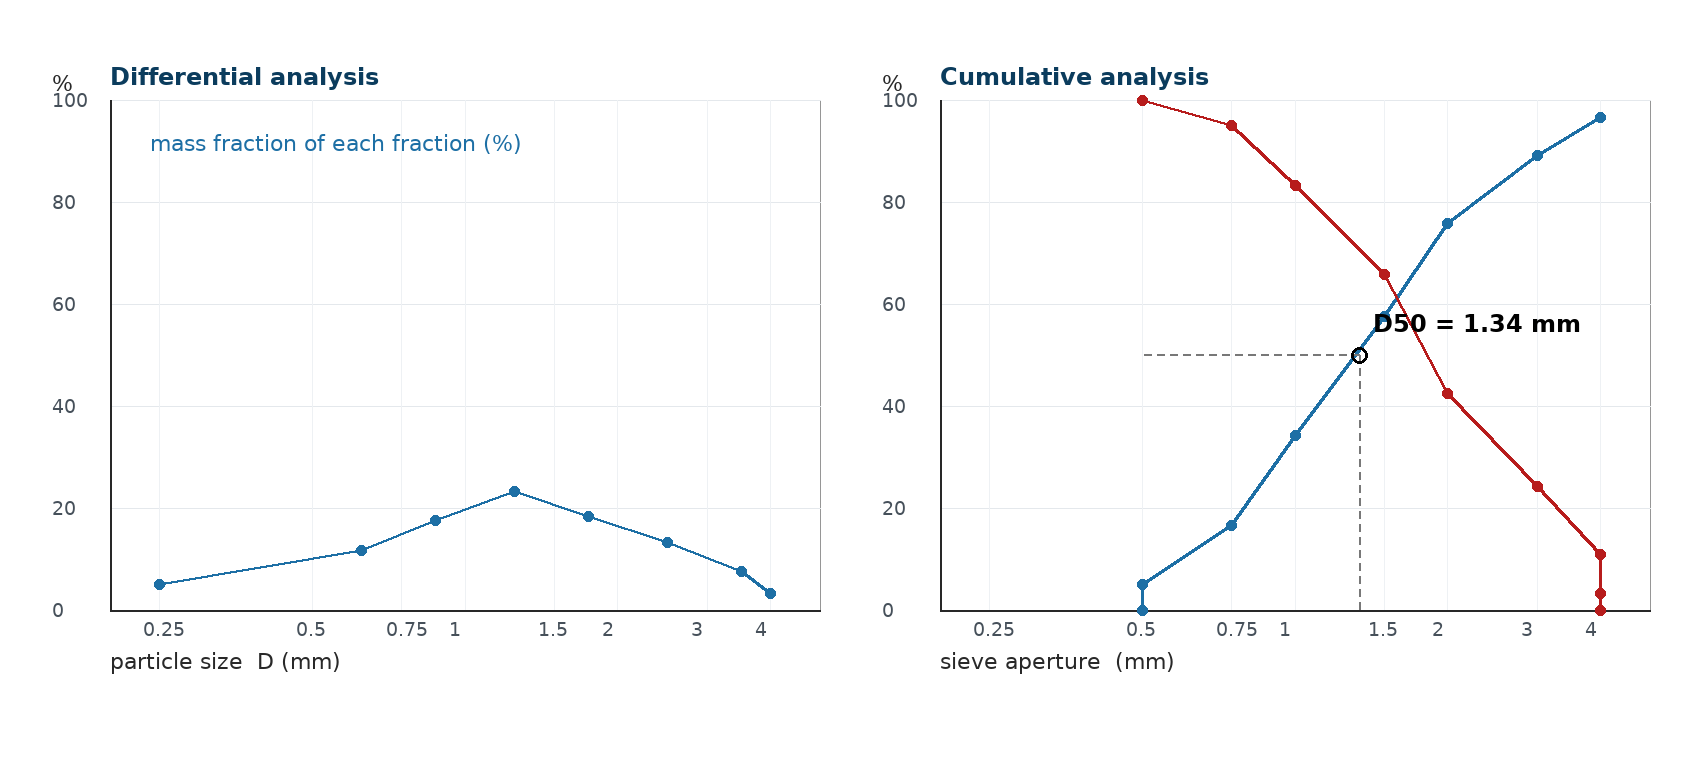
\includegraphics[width=\linewidth]{sp2-sizing-curves.png}
\end{center}
The differential curve peaks in the 1.50--1.00\,mm increment, and the cumulative passing curve
crosses 50\% between 1.50 and 1.00\,mm.

\textbf{4. $D_{50}$ by interpolation.} Between the 1.50\,mm and 1.00\,mm apertures the passing
percentage falls from 57.500 to 34.167, so
\[
D_{50}=1.50-\frac{57.500-50.000}{57.500-34.167}(1.50-1.00)=\SI{1.339}{\milli\meter}\approx\SI{1.34}{\milli\meter}
\]
(interpolating linearly on the logarithm of the aperture instead gives \SI{1.32}{\milli\meter} ---
the two agree to the precision of the data).

\textbf{5. Number of particles in each fraction.} With spherical particles, $a=\pi/6=0.5236$, and
$\rho_p=\SI{2500}{\kilogram\per\cubic\meter}=\SI{2.5e-3}{\gram\per\cubic\milli\meter}$:
{\small
\begin{tabular}{@{}S[table-format=1.3] S[table-format=1.4] S[table-format=7.0] S[table-format=5.1]@{}}
\toprule
{$\overline{D}_{pi}$ / \si{\milli\meter}} & {$x_i$} & {$N_i$ in the 600\,g sample} & {particles per gram}\\
\midrule
4.000 & 0.0333 & 239 & 0.4\\
3.500 & 0.0750 & 802 & 1.3\\
2.500 & 0.1333 & 3911 & 6.5\\
1.750 & 0.1833 & 15680 & 26.1\\
1.250 & 0.2333 & 54760 & 91.3\\
0.875 & 0.1750 & 119737 & 199.6\\
0.625 & 0.1167 & 219038 & 365.1\\
0.250 & 0.0500 & 1466772 & 2444.6\\
\bottomrule
\end{tabular}}
Total: $1.88\times10^{6}$ particles in the 600\,g sample, i.e.\ about 3135 particles per gram.
The count is dominated by the finest fraction, which holds 78\% of all the particles but only 5\% of
the mass.

\textbf{6. Specific surface area.} With $\Phi_s=1$ (spherical) and $\rho_p=\SI{2.5e-3}{\gram\per\cubic\milli\meter}$:
\[
\sum\frac{x_i}{\overline{D}_{pi}}=0.96119\ \text{mm}^{-1},\qquad
A_w=\frac{6}{(\num{2.5e-3})(1)}(0.96119)=\SI{2307}{\square\milli\meter\per\gram}
=\SI{23.1}{\square\centi\meter\per\gram}=\SI{2.31}{\square\meter\per\gram}
\]
The equivalent Sauter diameter of the whole sample is $\overline{D}_{vs}=1/0.96119=\SI{1.04}{\milli\meter}$.

\begin{ansbox}
1. Differential table above ($\sum x_i=1.000$); 2. cumulative table above;
3. curves above; 4. $D_{50}=\SI{1.34}{\milli\meter}$; 5. particle counts above, total
$1.88\times10^{6}$ in 600\,g ($\approx3135$ per gram); 6. $A_w=\SI{2307}{\square\milli\meter\per\gram}
=\SI{2.31}{\square\meter\per\gram}$.
\end{ansbox}

\begin{warnbox}
\textbf{Notes.}
\begin{itemize}
  \item The aperture list is read as the sieve stack; the 20\,g is the material retained on the
        4.00\,mm sieve, and the 30\,g is the pan fraction below 0.50\,mm. The size of the top fraction
        is not defined by the data (there is no coarser screen) and is taken here as 4.00\,mm; it
        carries only 3.3\% of the mass.
  \item ``Shape factor = 1'' is read as \emph{sphericity} $\Phi_s=1$, i.e.\ spherical particles, which
        is what the specific-surface formula needs. If the intended volume shape factor were instead
        $a=1$ (cubes), the surface-area answer is unchanged but the particle counts fall by the factor
        $0.5236$ (about $9.9\times10^{5}$ particles in 600\,g).
  \item $D_{50}$ depends on where it is read: linear interpolation on the passing curve gives
        1.34\,mm, interpolation on the logarithm of the aperture gives 1.32\,mm.
\end{itemize}
\end{warnbox}

\newpage
\qtitle{Q7 --- Shape factor and sphericity}{Tutorial 3 \textperiodcentered{}\label{q:7} slide 3 \textperiodcentered{} 01-09-2026}
\src{\texttt{Tutorials/Tutorial 3.pptx}, slide 3 (``Problem 2'')}

\begin{qbox}
``An irregular particle has a volume of $2.0\times10^{-9}$\,m\textsuperscript{3} and a surface area
of $5.5\times10^{-6}$\,m\textsuperscript{2}. Its characteristic diameter is 1.5\,mm. Calculate the
shape factor and the sphericity.''
\end{qbox}

\begin{mthbox}
\textbf{Method from the slides} (Mod 1 Lec 1, slides 9--15):
\[
D_{ps}=\sqrt{\frac{s_p}{\pi}},\qquad
D_{pv}=\Big(\frac{6v_p}{\pi}\Big)^{1/3},\qquad
D_{vs}=\frac{6v_p}{s_p},\qquad
\Phi_s=\frac{6v_p}{D_ps_p}=\frac{D_{vs}}{D_p}
\]
with $v_p$ the volume of one particle, $s_p$ its surface area and $D_p$ its nominal (characteristic)
diameter.
\end{mthbox}

\spsub{Solution}
With $v_p=2.0\times10^{-9}$\,m\textsuperscript{3}, $s_p=5.5\times10^{-6}$\,m\textsuperscript{2},
$D_p=\SI{1.5}{\milli\meter}=\SI{1.5e-3}{\meter}$:

\textbf{Shape factor} (volume shape factor, as used in Q1 and Q2):
\[
a=\frac{v_p}{D_p^{3}}=\frac{2.0\times10^{-9}}{(1.5\times10^{-3})^{3}}=0.593
\]

\textbf{Volume-surface (Sauter) diameter} of the particle:
\[
D_{vs}=\frac{6v_p}{s_p}=\frac{6(2.0\times10^{-9})}{5.5\times10^{-6}}
=\SI{2.18e-3}{\meter}=\SI{2.18}{\milli\meter}
\]

\textbf{Sphericity} by the relation on the slides:
\[
\Phi_s=\frac{6v_p}{D_ps_p}=\frac{1.2\times10^{-8}}{(\num{1.5e-3})(\num{5.5e-6})}=1.45
\]

\begin{ansbox}
$a=\dfrac{v_p}{D_p^{3}}=0.59$;\qquad $D_{vs}=\dfrac{6v_p}{s_p}=\SI{2.18}{\milli\meter}$;\qquad
$\Phi_s=\dfrac{6v_p}{D_ps_p}=1.45$.
\end{ansbox}

\begin{warnbox}
\textbf{Note --- the printed data cannot be right.} Sphericity is at most 1 by its definition
(the sphere has the smallest surface area for a given volume), so $\Phi_s=1.45$ is impossible. The
figures imply that the sphere of the same volume ($\SI{1.56}{\milli\meter}$ diameter) would have
\SI{7.68e-6}{\meter\squared} of surface, \emph{more} than the \SI{5.5e-6}{\meter\squared} quoted for
the irregular particle. Check the numbers with the instructor --- if the surface area is meant to be
$5.5\times10^{-5}$\,m\textsuperscript{2}, the same formula gives $\Phi_s=0.145$.
\end{warnbox}

\newpage
\spsection{PART B (continued) --- TUTORIAL 4}

\qtitle{Q8 --- Crusher power when capacity and product size change}{Tutorial 4 \textperiodcentered{}\label{q:8} slide 2 \textperiodcentered{} 07-09-2026}
\src{\texttt{Tutorials/Tutorial 4\_7\_9\_2026.pptx}, slide 2 (``Problem 1'')}

\begin{qbox}
``A certain crusher accepts the feed rock having a volume-surface mean diameter of 20\,mm and
discharges a product having a volume-surface mean diameter of 5\,mm. The power required to crush
1200\,kg/hr of material is 9.5\,kW. What would be the power consumption if the capacity is reduced
to 100\,kg/hr and the product size to 4\,mm? Assume mechanical efficiency to be same in both the
cases.''
\end{qbox}

\begin{mthbox}
\textbf{Method from the slides} (Mod 1 Lec 5, slide 19). The feed and product are given as mean
diameters, so the size-reduction laws that use mean diameters apply:
\[
\text{Rittinger:}\ \frac{P}{\dot m}=K_R\Big[\frac{1}{D_{Sb}}-\frac{1}{D_{Sa}}\Big],
\qquad
\text{Kick:}\ \frac{P}{\dot m}=K_K\ln\frac{D_{Sa}}{D_{Sb}}
\]
with $D_{Sa}$ the feed size and $D_{Sb}$ the product size. Since the mechanical efficiency is the
same in both duties, the constant ($K_R$ or $K_K$) determined from the first duty carries over to
the second.
\end{mthbox}

\spsub{Solution}
\textbf{First duty.} $\dot m_1=1200$\,kg/h $=1.2$\,t/h, so the specific energy is
\[
\frac{P_1}{\dot m_1}=\frac{9.5}{1.2}=\SI{7.9167}{\kilo\watt\hour\per\tonne}
\]
With $D_{Sa}=20$\,mm and $D_{Sb}=5$\,mm, the Rittinger size term is
$\frac{1}{5}-\frac{1}{20}=\SI{0.15}{\per\milli\meter}$, hence
\[
K_R=\frac{7.9167}{0.15}=\SI{52.78}{\kilo\watt\hour\milli\meter\per\tonne}
\]

\textbf{Second duty.} The same feed (20\,mm) is crushed to 4\,mm at $\dot m_2=100$\,kg/h
$=0.1$\,t/h:
\[
\frac{1}{4}-\frac{1}{20}=\SI{0.20}{\per\milli\meter},\qquad
P_2=K_R\,\dot m_2\Big[\frac{1}{D_{Sb}}-\frac{1}{D_{Sa}}\Big]
=(52.78)(0.1)(0.20)=\SI{1.06}{\kilo\watt}
\]

\begin{ansbox}
$K_R=\SI{52.78}{\kilo\watt\hour\milli\meter\per\tonne}$;\qquad
$P_2=\SI{1.06}{\kilo\watt}$ for 100\,kg/h to 4\,mm (Rittinger's law).
\end{ansbox}

\begin{warnbox}
\textbf{Notes.}
\begin{itemize}
  \item The question does not name the law. Rittinger's is used because the data are mean diameters,
        which is how the lecture's crusher problem (Q4) is set up. If Kick's law is intended instead,
        $K_K=7.9167/\ln(20/5)=\SI{5.711}{\kilo\watt\hour\per\tonne}$ and
        $P_2=5.711\ln(20/4)(0.1)=\SI{0.92}{\kilo\watt}$.
  \item Bond's law cannot be applied to these data as they stand: it needs the work index $W_i$ and
        the 80\%-passing sizes, neither of which is given here.
\end{itemize}
\end{warnbox}

\qtitle{Q9 --- Energy per kg of material}{Tutorial 4 \textperiodcentered{}\label{q:9} slide 3 \textperiodcentered{} 07-09-2026}
\src{\texttt{Tutorials/Tutorial 4\_7\_9\_2026.pptx}, slide 3 (``Problem 2'', printed inside a picture on the slide)}

\begin{qbox}
``A material is crushed from an initial particle size of 10\,mm to a final size of 2\,mm. If the
Kick's constant is 5\,kJ/kg, calculate the energy required per kg of material.''
\end{qbox}

\begin{mthbox}
\textbf{Method from the slides} (Mod 1 Lec 5, slide 19):
\[
\frac{E}{m}=K_K\ln\frac{D_{Sa}}{D_{Sb}}
\]
\end{mthbox}

\spsub{Solution}
\[
\ln\frac{10}{2}=\ln 5=1.6094,\qquad
\frac{E}{m}=5\times1.6094=\SI{8.05}{\kilo\joule\per\kilogram}
\]

\begin{ansbox}
$\dfrac{E}{m}=\SI{8.05}{\kilo\joule\per\kilogram}$ (i.e.\ 8.05\,kJ for every kg crushed).
\end{ansbox}

\newpage
\spsection{PART C --- TEST PAPERS}

\qtitle{Q10 --- Mixing index of a binary solid mixture}{Quiz-1 \textperiodcentered{}\label{q:10} 03-09-2026 \textperiodcentered{} 10 marks}
\src{\texttt{Tests/Quiz1\_Soln.pdf}, page 1 (question) and page 2 (the instructor's sample solution)}

\begin{qbox}
``A binary solid mixture consists of Component A and Component B. The overall composition of A in the
mixture is 50\% by mass. Samples are withdrawn from different locations after mixing. Each sample has
a total mass of 100\,g, and the mass of Component A in each sample is measured as follows:''
\begin{center}\small
\begin{tabular}{@{}l S[table-format=2.0] l S[table-format=2.0] l S[table-format=2.0] l S[table-format=2.0]@{}}
\toprule
{Sample} & {mass of A / \si{\gram}} & {Sample} & {mass of A / \si{\gram}} & {Sample} & {mass of A / \si{\gram}} & {Sample} & {mass of A / \si{\gram}}\\
\midrule
1 & 52 & 4 & 45 & 7 & 54 & 10 & 50\\
2 & 48 & 5 & 51 & 8 & 46 & & \\
3 & 55 & 6 & 49 & 9 & 50 & & \\
\bottomrule
\end{tabular}
\end{center}
``Assuming each 100-g sample contains 1000 particles. Calculate the mixing index.''
\end{qbox}

\begin{mthbox}
\textbf{Method from the slides} (Mod 1 Lec 4, slides 16--18):
\[
s=\sqrt{\frac{\sum_{i=1}^{N}x_i^2-\bar x\sum_{i=1}^{N}x_i}{N-1}},
\qquad
\sigma_0=\sqrt{\mu(1-\mu)},
\qquad
I_s=\frac{\sigma_0}{s}
\]
with $x_i$ the mass fraction of A in each sample and $\mu$ the overall mass fraction of A.
\end{mthbox}

\spsub{Solution}
The mass fractions are $x_i=0.52,0.48,0.55,0.45,0.51,0.49,0.54,0.46,0.50,0.50$;
\[
\sum_{i=1}^{10}x_i=5.0000,\qquad \sum_{i=1}^{10}x_i^2=2.5092,\qquad \bar x=0.5000
\]
\[
s=\sqrt{\frac{2.5092-(0.5)(5.0)}{10-1}}=\sqrt{\frac{0.0092}{9}}=0.03197
\]
\[
\sigma_0=\sqrt{0.5\times0.5}=0.50,\qquad
I_s=\frac{\sigma_0}{s}=\frac{0.50}{0.03197}=15.6
\]

\begin{ansbox}
$\bar x=0.5000$;\quad $s=0.0320$;\quad $\sigma_0=0.50$;\quad $\boxed{I_s=15.6}$.
\end{ansbox}

\note{The sample solution in the file rounds $s$ to 0.031 and reports $I_s=0.5/0.031=16.1$; the
difference is only that rounding. Two variants, for completeness: with the $N$ denominator
$s=0.03033$ and $I_s=16.5$; if the 1000 particles per sample are used in the granular form
$\sigma_e=\sqrt{\mu_p(1-\mu_p)/n}=\sqrt{0.25/1000}=0.0158$, then $I_s=\sigma_e/s=0.49$, which is the
form used for non-cohesive granular solids on slide 17. The mixture here is sampled by mass and the
question gives a mass composition, so the mass-based $\sigma_0$ of slide 18 is the one used above.}

\qtitle{Q11 --- Bond work index and power for a finer product}{Tutorial Test 1 \textperiodcentered{}\label{q:11} 07-09-2026 \textperiodcentered{} 15 marks}
\src{\texttt{Tests/TT1\_Solution.pdf}, page 1 (question) and pages 1--2 (the instructor's solution)}

\begin{qbox}
``320\,kW of power is required to crush 140 tonnes/h of a material. If 80\% of the feed passes
through a 50-mm screen and 80\% of the product passes through a 2-mm screen, calculate the work index
of the material. What will be the power required for the same feed at 140 tonnes/h to be crushed to a
product such that 80\% is to pass through a 1.6-mm screen?''
\end{qbox}

\begin{mthbox}
\textbf{Method from the slides} (Mod 1 Lec 5). Bond's law as given on slide 19, with the work index
defined on slide 17 as the energy needed to take a very large feed to a product 80\% passing
\SI{100}{\micro\meter}:
\[
\frac{P}{\dot m}=0.3162\,W_i\Big[\frac{1}{\sqrt{D_{pb}}}-\frac{1}{\sqrt{D_{pa}}}\Big]
\qquad (D\ \text{in \si{\milli\meter}},\ P/\dot m\ \text{in \si{\kilo\watt\hour\per\tonne}})
\]
\end{mthbox}

\spsub{Solution}
\textbf{1. Work index from the first duty.} $\dot m_1=\SI{140}{\tonne\per\hour}$, so
\[
\frac{P_1}{\dot m_1}=\frac{320}{140}=\SI{2.2857}{\kilo\watt\hour\per\tonne}
\]
Here $D_{pa}=50$\,mm and $D_{pb}=2$\,mm (the 80\%-passing sizes):
\[
\frac{1}{\sqrt{2}}-\frac{1}{\sqrt{50}}=0.70711-0.14142=0.56569
\]
\[
W_i=\frac{2.2857}{0.3162\times0.56569}=\SI{12.78}{\kilo\watt\hour\per\tonne}
\]

\textbf{2. Power for the finer product.} Now $D_{pb}=1.6$\,mm at the same feed (50\,mm) and the same
140 tonnes/h:
\[
\frac{1}{\sqrt{1.6}}-\frac{1}{\sqrt{50}}=0.79057-0.14142=0.64915
\]
\[
\frac{P_2}{\dot m}=0.3162(12.78)(0.64915)=\SI{2.623}{\kilo\watt\hour\per\tonne},
\qquad
P_2=2.623\times140=\SI{367.2}{\kilo\watt}
\]

\begin{ansbox}
$W_i=\SI{12.78}{\kilo\watt\hour\per\tonne}$;\qquad
$\boxed{P_2=\SI{367.2}{\kilo\watt}}$ (specific energy \SI{2.62}{\kilo\watt\hour\per\tonne}).
\end{ansbox}

\note{This agrees with the boxed values in the instructor's solution (12.78 and 367.22\,kW). Note
that the \SI{320}{\kilo\watt} is the total power drawn; unlike Q4, no empty-mill allowance is given
here, so no deduction is made.}

\spsection{PART D --- MODULE 2 PROBLEMS (from \texttt{Problems.pptx} and the Lec.~8 deck)}

\qtitle{Q12 --- Capacity of a clarifying centrifuge}{Module 2 \textperiodcentered{}\label{q:12} Lecture 8 \textperiodcentered{} slide 26}
\src{\texttt{Slides/Mod 2-Lecture 8-compressed.pdf}, slide 26 (``Problem on Centrifugal Sedimentation'')}

\begin{qbox}
``What is the capacity in cubic meters per hour of a clarifying centrifuge operating under the
following conditions?'' Bowl diameter \SI{600}{mm}; thickness of liquid layer \SI{75}{mm}; depth of
bowl \SI{400}{mm}; speed \SI{1200}{r/min}; specific gravity of liquid 1.2; specific gravity of solid
1.6; viscosity of liquid \SI{2}{cP}; cut size of particles \SI{30}{\micro\meter}.
\end{qbox}

\begin{mthbox}
\textbf{Method from the slides} (Mod 2 Lec 8, slide 26): the cut-point equation printed on that slide,
\[
q_c=\frac{\pi b\,\omega^{2}(\rho_p-\rho)D_{pc}^{2}}{18\mu}\,
    \frac{r_2^{2}-r_1^{2}}{\ln\left[\dfrac{2r_2}{r_1+r_2}\right]}
\]
with $b$ the bowl depth, $r_1$ and $r_2$ the inner radii of the liquid layer and of the bowl, and
$D_{pc}$ the cut size.
\end{mthbox}

\spsub{Data in consistent units}
$r_2=\SI{0.300}{m}$; liquid layer \SI{75}{mm} thick, so $r_1=0.300-0.075=\SI{0.225}{m}$;
$b=\SI{0.400}{m}$; $\rho_p=1600$ and $\rho=1200$~kg/m$^3$ (specific gravities 1.6 and 1.2);
$\mu=2$~cP $=\SI{0.002}{Pa.s}$; $D_{pc}=\SI{30e-6}{m}$; and
\[
\omega=\frac{2\pi(1200)}{60}=\SI{125.66}{rad/s},\qquad \omega^{2}=\SI{15791}{rad^2/s^2}
\]

\spsub{Solution --- the slide's cut-point equation}
Particle term:
\[
\frac{\pi b\,\omega^{2}(\rho_p-\rho)D_{pc}^{2}}{18\mu}
=\frac{\pi(0.4)(15791)(400)(9\times10^{-10})}{0.036}
=\SI{0.19844}{m^3/s}
\]
Geometry term:
\[
\frac{r_2^{2}-r_1^{2}}{\ln[2r_2/(r_1+r_2)]}
=\frac{0.09-0.050625}{\ln[0.6/0.525]}
=\frac{0.039375}{0.13353}=0.29487
\]
\[
q_c=0.19844\times0.29487=\SI{0.058515}{m^3/s}
\]

\begin{ansbox}
$\boxed{q_c=\SI{210.7}{m^3/h}}$ (equivalently \SI{0.0585}{m^3/s}).
\end{ansbox}

\note{Cross-check with the other form the deck carries for the same problem, the thin-liquid-layer
result $q_c=\dfrac{2V\omega^{2}r_2D_p^{2}(\rho_p-\rho)}{18\mu s}$ of slide 23, using
$V=\pi b(r_2^{2}-r_1^{2})=\SI{0.04948}{m^3}$ and $s=\SI{0.075}{m}$: this gives
\SI{225.0}{m^3/h}, about 6.8\,\% higher, which is what the thin-layer approximation is expected to
do. The cut-point equation of slide 26 (with $r_A=(r_1+r_2)/2$) is the one printed with the problem
and is the answer quoted.}

\qtitle{Q13 --- Mill speed when the grinding balls are replaced}{Module 1 \textperiodcentered{}\label{q:13} Lecture 6 (critical-speed relation), from \texttt{Problems.pptx} slide 2}
\src{\texttt{Slides/Problems.pptx}, slide 2}

\begin{qbox}
``In a ball mill of 2000-mm diameter, 100-mm diameter steel balls are being used for grinding.
Presently for the material being ground, the mill is running at 15 rpm. At what speed will the mill
have to run if the 100-mm balls are replaced with 50-mm balls, all the other conditions remaining
same?''
\end{qbox}

\begin{mthbox}
\textbf{Method from the slides} (Mod 1 Lec 6): the critical speed of a ball mill, in revolutions per
second,
\[
n_c=\frac{1}{2\pi}\sqrt{\frac{g}{R-r}}
\]
with $R$ the radius of the mill and $r$ the radius of the grinding elements. A mill is run at a fixed
fraction of its critical speed (65--80\,\%, from the same slide), so that fraction is what is held
constant when the ball size changes.
\end{mthbox}

\spsub{Solution}
$R=1.000$~m; the original balls have $r=0.050$~m, so $R-r=0.950$~m:
\[
n_{c,1}=\frac{1}{2\pi}\sqrt{\frac{9.81}{0.950}}=0.51144\ \text{rev/s}=30.69\ \text{rpm}
\]
The mill runs at \SI{15}{rpm}, that is
\[
\frac{n_1}{n_{c,1}}=\frac{15}{30.69}=0.4888
\]
For 50-mm balls, $r=0.025$~m and $R-r=0.975$~m:
\[
n_{c,2}=\frac{1}{2\pi}\sqrt{\frac{9.81}{0.975}}=0.50484\ \text{rev/s}=30.29\ \text{rpm}
\]
Keeping the same fraction of critical speed,
\[
n_2=0.4888\times30.29=\SI{14.81}{rpm}
\]
and the same result directly: $n_2=n_1\sqrt{(R-r_1)/(R-r_2)}=15\sqrt{0.950/0.975}$.

\begin{ansbox}
$\boxed{n_2=\SI{14.8}{rpm}}$ --- slightly slower than the present \SI{15}{rpm}: smaller balls raise the
critical speed only a little, and the operating point (the same fraction of critical speed) is
unchanged.
\end{ansbox}

\qtitle{Q14 --- Washing time and doubled filter area in a plate-and-frame press}{from \texttt{Problems.pptx}, slides 3--4 \textperiodcentered{}\label{q:14}}
\src{\texttt{Slides/Problems.pptx}, slide 3 (question) and slide 4 (the deck's own worked solution)}

\begin{qbox}
``A sludge filtered in a washing plate and frame filter press is of such nature that the filtration
equation is $V^{2}=Kt$ where $V$ is the volume of filtrate obtained in time $t$, when the pressure is
constant. \SI{30}{m^3} of filtrate is produced in 10 hours. \SI{3}{m^3} of wash water is forced
through the cake at the end of filtration. (a) What is the length of the washing time? (b) If the
filtering surface of the press is doubled, all other conditions remaining constant, how long would it
take to produce \SI{30}{m^3} of filtrate?''
\end{qbox}

\begin{mthbox}
\textbf{Method: the deck's own solution slide}, using $V^{2}=Kt$ (constant pressure) together with the
cake-resistance group of Mod 2 Lec 4/5: $K=\dfrac{A^{2}\Delta P^{\,1-s}}{Z}$ with
$Z=\mu\alpha_0c/2$ a constant, and
\[
\frac{\mathrm{d}t}{\mathrm{d}V}=\frac{\mu}{A\Delta P}\Big(\alpha c\,\frac{V}{A}+R_m\Big)
\qquad\text{filter-medium resistance $R_m$ neglected, as the slide does.}
\]
\end{mthbox}

\spsub{Solution (a) --- washing time}
From the run, $V=\SI{30}{m^3}$ in $t=\SI{10}{h}$:
\[
K=\frac{V^{2}}{t}=\frac{30\times30}{10}=\SI{90}{m^6/h}
\]
Rate of filtration at the end of the run:
\[
\frac{\mathrm{d}V}{\mathrm{d}t}=\frac{K}{2V}=\frac{90}{2\times30}=\SI{1.5}{m^3/h}
\]
Washing rate of a plate-and-frame press $=\tfrac14\times$ rate of filtration $=\SI{0.375}{m^3/h}$
(one quarter, because only a quarter of the flow path is available to the wash water in a frame
press), so
\[
t_w=\frac{\text{volume of wash water}}{\text{rate of washing}}=\frac{3}{0.375}=\SI{8}{h}
\]

\spsub{Solution (b) --- filtering surface doubled}
With $A'=2A$ and everything else unchanged ($\Delta P$, $s$, $Z$ constant),
\[
K'=\frac{A'^{2}\Delta P^{\,1-s}}{Z}=\frac{(2A)^{2}\Delta P^{\,1-s}}{Z}=4K
=4\times90=\SI{360}{m^6/h}
\]
and the same \SI{30}{m^3} is now obtained in
\[
t'=\frac{V^{2}}{K'}=\frac{30^{2}}{360}=\SI{2.5}{h}
\]

\begin{ansbox}
(a) $t_w=\SI{8}{h}$;\qquad (b) $t'=\SI{2.5}{h}$ (a quarter of the original time, because $K\propto A^{2}$).
\end{ansbox}

\note{Both answers are the deck's own boxed results (8 hours and 2.5 hours). The $V^{2}=Kt$ form of
the filtration equation is the one the question itself states; the deck's solution reloads it for the
new area through $K\propto A^{2}$, which is what makes part (b) a quarter of the original time.}

\qtitle{Q15 --- Purity of dressed ore from a hydraulic classifier}{from \texttt{Problems.pptx}, slide 5 (Example 6.3) \textperiodcentered{}\label{q:15}}
\src{\texttt{Slides/Problems.pptx}, slide 5}

\begin{qbox}
``An ore sample having a specific gravity of 2.1 is to be separated from rock associated with it
using a hydraulic classifier. The ore consists of 1~mm spherical particles. The rock particles have
an average specific gravity of 5.4 and the screen analysis gives the following:

\begin{center}
\begin{tabular}{@{}lc@{}}
\toprule
Particle size / \si{\milli\meter} & Mass fraction\\
\midrule
$+2-5$ & 0.43\\
$+0.5-2$ & 0.47\\
$<0.5$ & 0.10\\
\bottomrule
\end{tabular}
\end{center}

The ore--rock mixture contains 30\,\% rock particles. Estimate the \,\% purity of the dressed ore.
Assume settling to be laminar.''
\end{qbox}

\begin{mthbox}
\textbf{Method from the slides} (Mod 2 Lec 7, differential settling; Stokes' law regime): equal-settling
particles of two materials A and B in a medium of density $\rho$ are related by
\[
\frac{D_A}{D_B}=\sqrt{\frac{\rho_B-\rho}{\rho_A-\rho}}
\qquad\text{so}\qquad
D_{rock}=D_{ore}\sqrt{\frac{\rho_{ore}-\rho}{\rho_{rock}-\rho}}
\]
With \SI{1}{mm} ore particles in water (\SI{1000}{kg/m^3}),
\[
D_{rock}=1\times\sqrt{\frac{2.1-1}{5.4-1}}=1\times\sqrt{\frac{1.1}{4.4}}=\SI{0.5}{mm}
\]
so a \SI{1}{mm} ore particle settles at exactly the same rate as a \SI{0.5}{mm} rock particle.
\end{mthbox}

\spsub{Reading the classification}
Set the classifier so that no ore is lost --- the cut velocity is the terminal velocity of a \SI{1}{mm}
ore particle:
\begin{itemize}
  \item rock \emph{coarser} than the equal-settling size \SI{0.5}{mm} settles faster than the ore and is
        retained with it: the $+2-5$ and $+0.5-2$ fractions, $0.43+0.47=0.90$ of the rock;
  \item rock \emph{finer} than \SI{0.5}{mm} settles more slowly and is carried away in the overflow,
        the remaining $0.10$ of the rock.
\end{itemize}
Per unit mass of the ore--rock mixture: ore $=0.70$, rock $=0.30$, of which retained
$=0.90\times0.30=0.270$. Therefore
\[
\text{purity}=\frac{\text{ore}}{\text{ore}+\text{retained rock}}
=\frac{0.70}{0.70+0.27}=\frac{0.70}{0.97}=0.7216
\]

\begin{ansbox}
$\boxed{\text{purity}\approx72\,\%}$ --- in one pass at the \SI{1}{mm} cut the dressed ore is 72.2\,\%
ore, the balance being rock of \SI{0.5}{mm} and coarser that settles with it.
\end{ansbox}

\begin{warnbox}
\textbf{Where this problem is under-specified, and what was assumed.} The slide prints the screen
analysis after naming the rock, so the fractions are read as the \emph{rock's} own size distribution
(the ore is stated separately as \SI{1}{mm} particles). Read instead as the size distribution of the
\emph{mixture}, the same numbers cannot hold: with 30\,\% rock the mixture would be 70\,\% ore, yet the
whole of the ore would have to lie inside the $+0.5-2$ fraction, which is only 47\,\% of the mixture.
The slide gives no worked answer, so the cut is stated explicitly above (no ore lost) and the answer
is quoted for that cut; another cut gives another purity, and the last line of the calculation is
redone in one step: $\text{purity}=0.70/(0.70+0.90x)$ with $x$ the retained fraction of the rock.
\end{warnbox}

\vspace{2mm}
{\color{rule}\hrule height 0.6pt}
\vspace{2mm}
\note{Questions, data and methods: the uploaded files listed under each question. Arithmetic: every
number above is reproduced by \texttt{sp2-answers-check.py} in this folder, which is the record of
the calculations. Where a source is silent or contradicts itself, the note under that solution says
so.}

\end{document}
